\documentclass{deliverablereport}

\deliverable{dissem}{ibook1}
\deliverydate{31/08/2018}
\duedate{31/08/2018 (M36)}
\author{Marcin Kostur, Jerzy Łuczka, Jan Aksamit, Jolanta Marzec}

\begin{document}
\maketitle


% \githubissuedescription

\section{Introduction}

Interactive webpages have always been an attractive tool in
education. It has started in the age of Adobe-Flash technology, when a
lot of educational materials have been created. The advent of
javascript has led to significant improvements in that field: in the
first place it created a possibility to author the content with
Open Source tools and secondly it increased the portability to
practically all devices equipped with modern web browser.

The problems which was persistent in those solutions was the big gap
between the authoring process of interactive tools and their
usage. Usually the code behind of interactive examples was not very
educational and was not supposed to be edited by the student. On the
other hand Open Source tools such as \Sage, delivered a versatile
solution to this problem. Pricipally, the \texttt{@interact} decorator
has made possibile to convert a scientific calculation into web-based
interactive application. The biggest advantage of this solution is
that one can create a visually appealing scintific interaction using
the same environment in which the mathematical exlorations took place.

The source code of interactive books is hosted on github within
OpenDreamKit organization in
\href{https://github.com/OpenDreamKit/iODKbook2}{iODKbook2 repository}.


\section{Interactive book technology}

We have used well known in Python community \Sphinx documentation
generator for the main authoring tool. \Sphinx contains plugins system,
which allows specialize it for a particular application. In our case
we will apply extenstion able to: 

\begin{itemize}
\item embedd \Sage code and allow for interactive execution on a
  remote server using SageMathCell technology (see
  fig. \ref{fig:interact_sphinx}).
\item use conditional compilation of parts depending e.g. if target
  medium is interactive of not.
\item include automatically \Jupyter notebooks with embedded output
\item produce high quality pdf via \LaTeX system.
\end{itemize}  


In the authoring process one can produce notebook (sagenb or \Jupyter
based) and decide if it should be included into the \Sphinx book or
choose selected examples and influde them as live SageCellServer code
which can be used interactively. It has to be stressed that not only
elemnents having \texttt{@interact} are usefull. Practically all
excercises can be done inside the book in the interactive code
boxes. It is reasonable, however, to limit the reader to write only
short pieces of code in this way, because the code written in browser
without login is volatile and can dissappear if one reloads the page.

\begin{figure}
\centerline{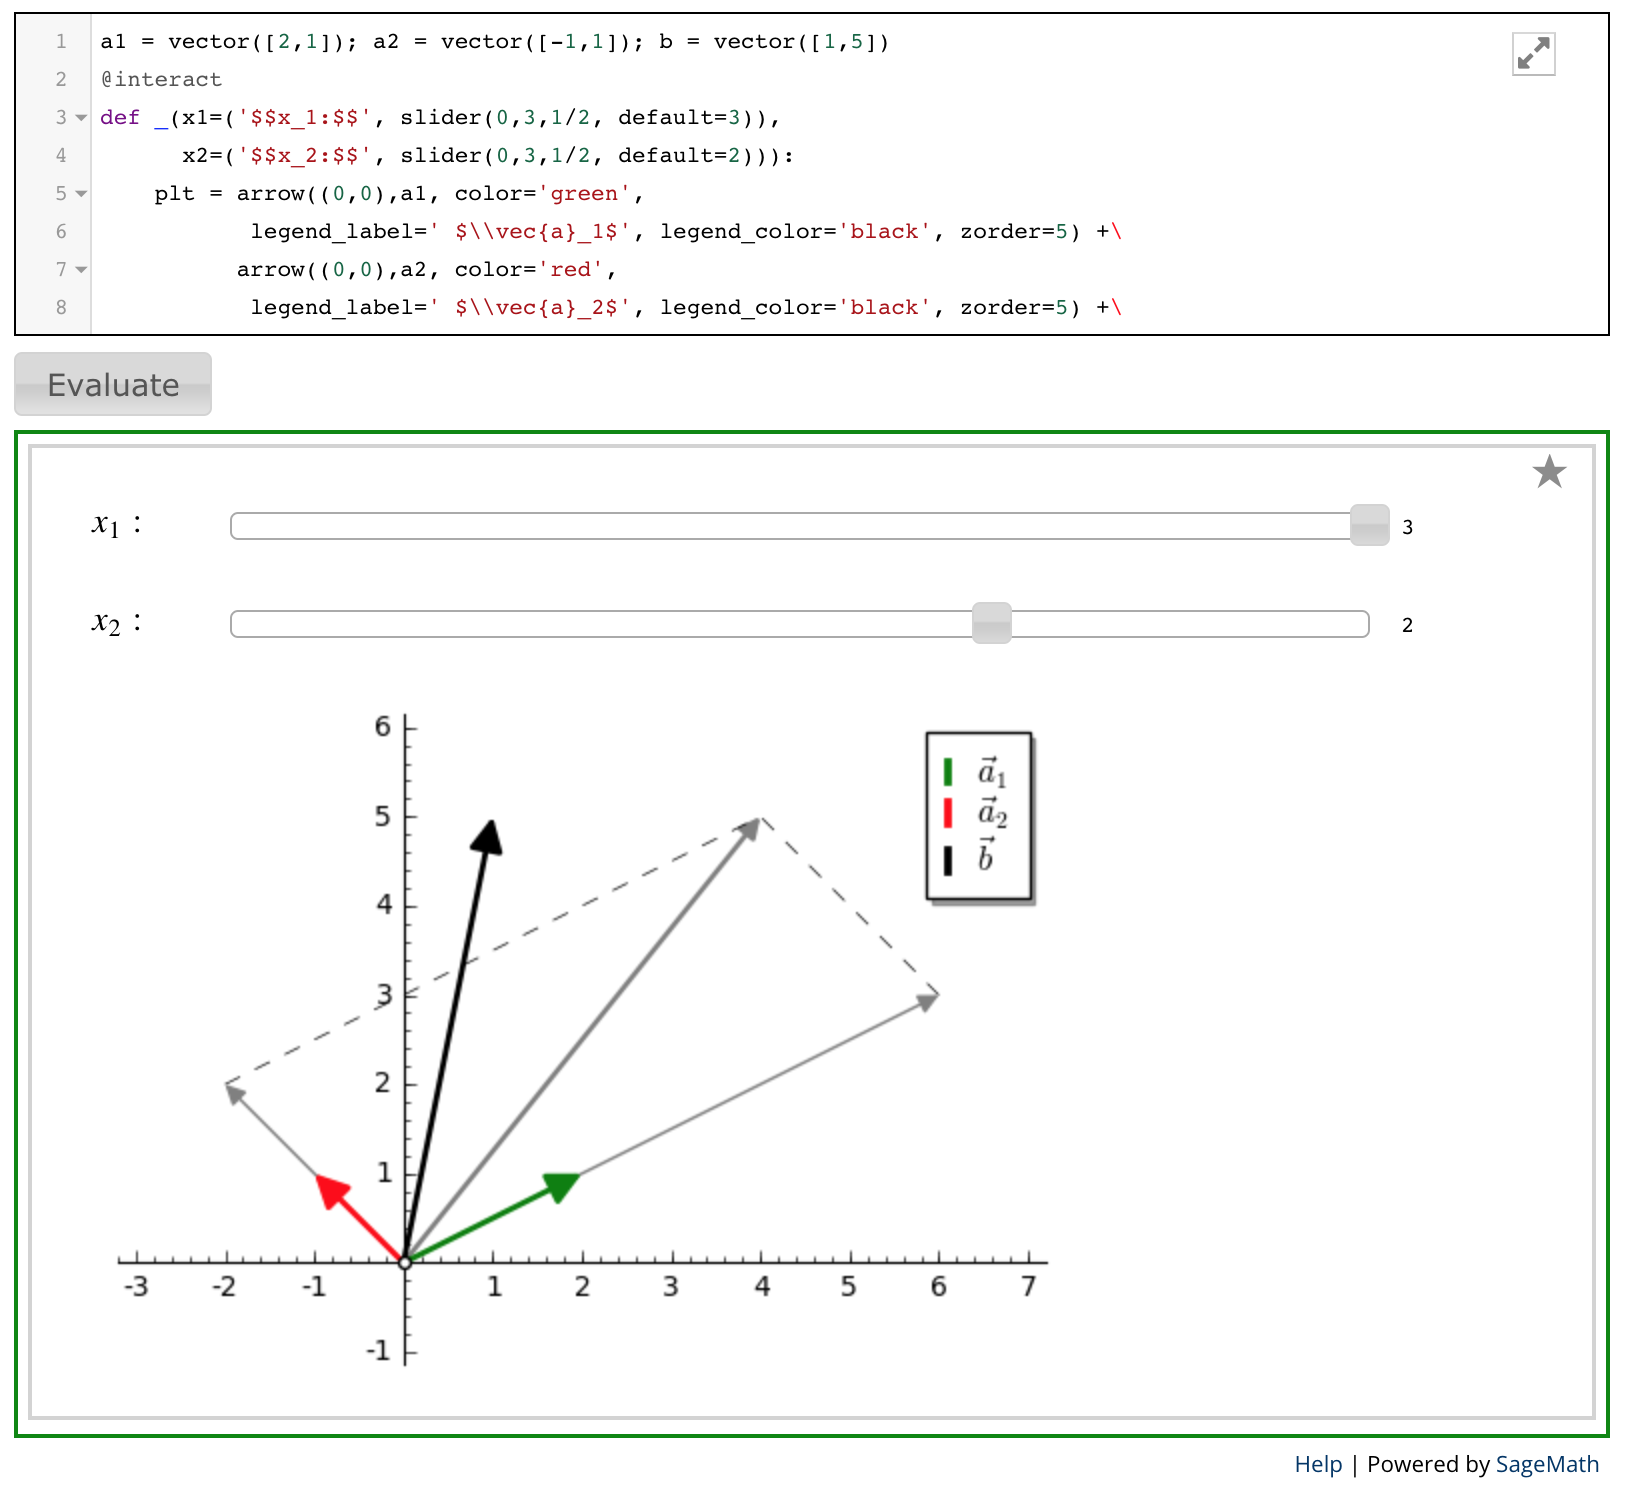
\includegraphics[width=.7\textwidth]{interact_in_sphinx.png}}
\caption{\label{fig:interact_sphinx} An example of \texttt{@interact} in
  \Sphinx generated web version of interactive book. The upper box
  shows the code and the lower box shows the output.}
\end{figure}


\section{ Nonlinear Processes in Biology }


The book is in large extend based on coursework taught at University
of Silesia. It was primarily based on sagenb system and gradually was
converted into the interactive book with live examples.


The book covers the classical topics in modeling in
biology. Methodologically it can be split into following groups:

\begin{enumerate}
\item Methods of mathematical modelling of  processes based on ODE and PDE. 
\item Qualitative methods in ODE and PDE with application of Sage. It
  includes:
  \begin{itemize}
  \item stationary states of the system,
  \item the linear stability of fix points,
  \item phase curves,
  \item bifurcation diagrams,
  \item time-dependent solutions,
  \item a graphical  presentation of all above  elements. 
  \end{itemize}
  
  To each subject there is a list of related problems and
  supplementary tasks as homework. All requires symbolic manipulations
  as well as certain techniques from numerical analysis like root
  finding.
  
\item Numerical solving of ODEs. It is complementary to analytical and
  qualitative methods for ODE. 
\item Numerical solving of PDE-s - diffusion equation,
  reaction-diffusion systems and similar. It requires good tools in data
  processing, usually uses numpy for calculations.

\end{enumerate}


It turned out that conceptually simple methods - like plotting a
function of one variable, which depends on a parameter (see
fig. \ref{fig:interact2}), can be very usefull for the analysis of
models containing analytically untractable expressions. In this
particular example, students can construct just a simple plot of a
function, and with a help of \texttt{@interact} construction it can be
easily converted intro an applet which allow for ananlysis of the
system. 

The book covers the following  models: 
 \begin{itemize}
  \item one-dimensional systems (Malthus, Verhulst, Ludwig, Alee models) 
  \item two-dimensional systems (Lotka-Volterra, May models) 
  \item kinetics of chemical reactions
  \item Belousov-Zhabotinsky reactions
  \item models of epidemics
 \end{itemize}

\begin{figure}
\centerline{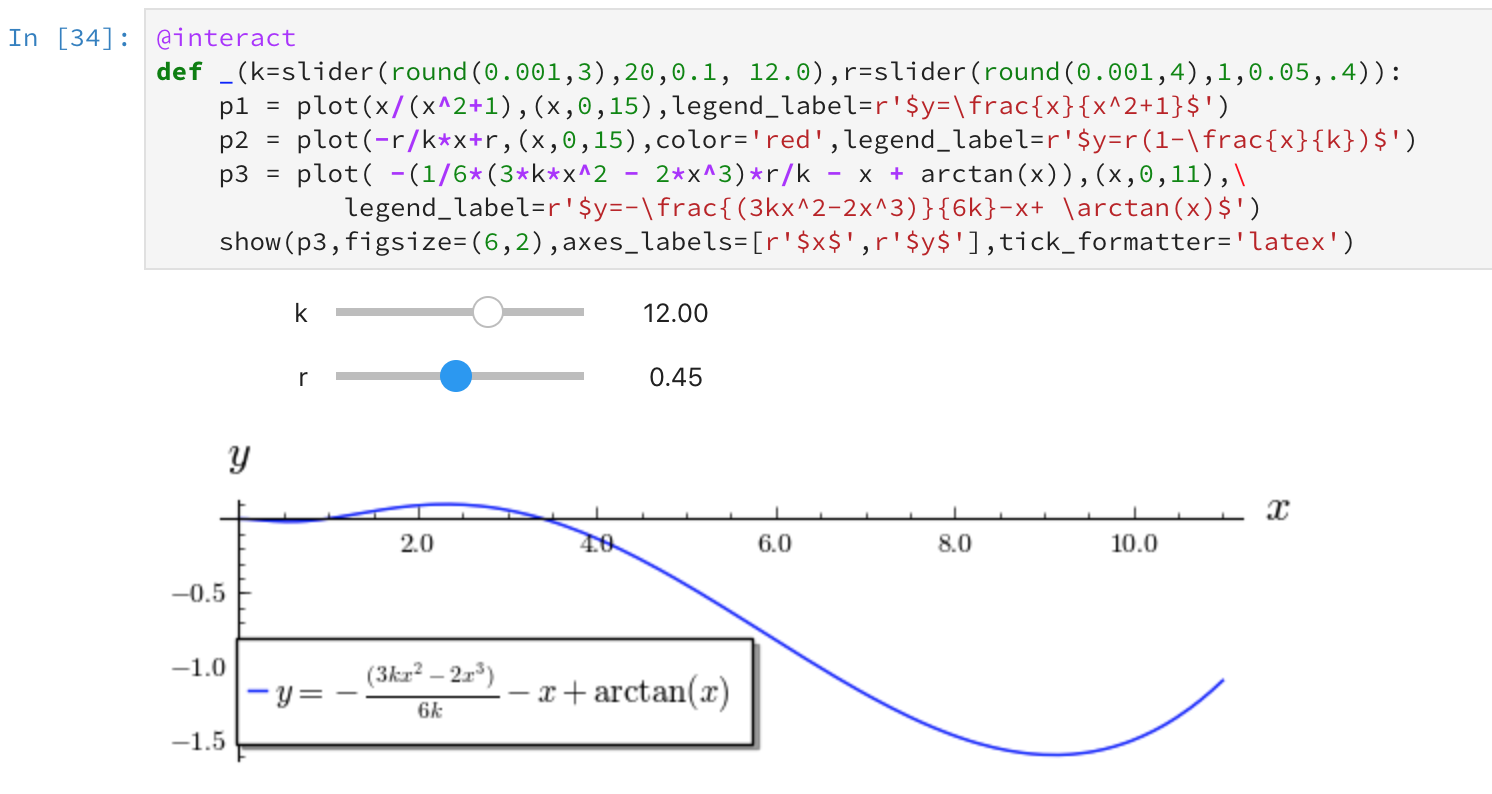
\includegraphics[width=.7\textwidth]{interact_npb.png}}
\caption{\label{fig:interact2} An example of \texttt{@interact}
  applied for graphical examination of roots of a function. It is a
  first step in qualitative analysis of model of tumor growth in a
  book.  }
\end{figure}







\subsection{Lectures on Linear Algebra}

This book is based on courses of linear algebra for physics students
taught in recent years at the University of Silesia. It has been
gradually equipped with interactive materials and extended by sections
illustrating application of linear algebra in economy, computer
science and other areas. The computations and the interactive part are
performed by \Sage, which is embedded in the book.

Along the theory the user becomes familiar with the code used in
\Sage. Their learning process is enhanced by various factors:
\begin{itemize}
\item numerous visualisations;
\item interactive images which allow construction of a graphical
  solution to a problem; this problem may be changed in real time by
  the user by changing the code;
\item place for experiments: the user may fill in the gaps in the code
  to produce graphical interpretation of a chosen operation;
\item possibility to perform the calculations with \Sage within the
  book; in particular, computations with real data and, thus, real
  life conclusions are possible;
\item some longer coding exercises are equipped with the check points
  (without revealing the answer) to ensure that the solution is
  correct.
\end{itemize}

Moreover, not only users benefits from interactive resources, but also
can learn how to produce them themselves.


\section{Future work}

The open texbooks are updated continously. We plan to add new models
or excercises on regular basis. Also there are efford being done to
encourage other lecturers to use contribute those materials.

\end{document}

%%% Local Variables:
%%% mode: latex
%%% TeX-master: t
%%% End:

